\section{Results}
\label{sec:results}
\label{sec:training-results}

\subsection{What throughput do the end-to-end routes achieve?}

The fastest custom path, \mxfp{} with row-gradient SR, reaches 37,876.8
tokens/s/GPU, compared with
18,812.0 for BF16 and 27,622.0 for TE-native \nvfp{} in all blocks.
Table~\ref{tab:gb200-throughput} reports the complete same-accelerator panel.
Every row uses sequence length 8,192, global batch 512, a BF16 output
projection, compiled regular CE, and a cross-device median over steps 40--100.
BF16 and TE use LB2/GA8; the custom paths use LB4/GA4.

\begin{table}[H]
  \centering
  \caption{GB200 throughput with compiled regular CE. Values are cross-device
  medians over steps 40--100 for each route's selected batch geometry. BF16
  uses selective-8 activation checkpointing; all other rows use selective-32.
  BF16 MFU uses NVIDIA's 2,500-TFLOP/s/GPU maximum dense BF16 throughput:
  180 PFLOP/s dense for 72 GPUs \cite{nvidia2025blackwell}.}
  \label{tab:gb200-throughput}
  \begin{adjustbox}{max width=\textwidth}
  \begin{tabular}{ll@{\qquad}rrr}
    \toprule
    Route & LB/GA & Tokens/s/GPU & BF16 MFU & Median HBM \\
    \midrule
    BF16 & 2/8 & 18,812.00 & 43.58\% & 101.19 GiB \\
    TE-native \nvfp{} in all blocks & 2/8 & 27,622.00 & 63.99\% & 125.80 GiB \\
    TE \nvfp{} + four final BF16 blocks & 2/8 & 27,077.50 & 62.73\% & 126.03 GiB \\
    Global \nvfp{} v5 & 4/4 & 32,490.50 & 75.27\% & 155.63 GiB \\
    \mxfp{} + row-SR & 4/4 & 37,876.75 & 87.74\% & 154.43 GiB \\
    \localcta{}-v4 & 4/4 & 33,243.76 & 77.01\% & 115.52 GiB \\
    \localcta{} + fixed H16 & 4/4 & 31,882.61 & 73.86\% & 114.89 GiB \\
    27/5 depth hybrid & 4/4 & 33,120.50 & 76.73\% & 126.21 GiB \\
    Operand hybrid + plain H16 & 4/4 & 34,782.50 & 80.58\% & 154.92 GiB \\
    Operand hybrid + fixed H32 & 4/4 & 35,085.50 & 81.28\% & 150.89 GiB \\
    \mxfp{} + row-SR + fixed H32 & 4/4 & 37,247.00 & 86.29\% & 151.02 GiB \\
    \bottomrule
  \end{tabular}
  \end{adjustbox}
\end{table}

Under the same world-32 LB4/GA4 geometry, the
\mxfp{}+row-SR+fixed-H32 route reaches 98.34\% of the row-SR-only \mxfp{} throughput.
Additional measurement details appear in
Appendix~\ref{app:implementation}.

\subsection{How closely do the recipes track BF16 training loss?}

Figure~\ref{fig:llama8b-loss} compares the training trajectories. The top panel
shows an exponential moving average over 31 logged observations (EMA-31). The
bottom panel follows the
relative-difference convention used by NVIDIA
\cite{nvidia2025nvfp4}:
\begin{equation}
  \Delta_{\mathrm{BF16}}(t)=100
  \frac{L_{\mathrm{BF16}}(t)-L_{\mathrm{route}}(t)}
       {L_{\mathrm{BF16}}(t)}.
  \label{eq:relative-loss}
\end{equation}
Zero is the BF16 reference and a negative value means the low-precision route
has higher loss. Curves are compared only at exact shared logged steps; no
loss value is interpolated.

\begin{figure}[tbp]
  \centering
  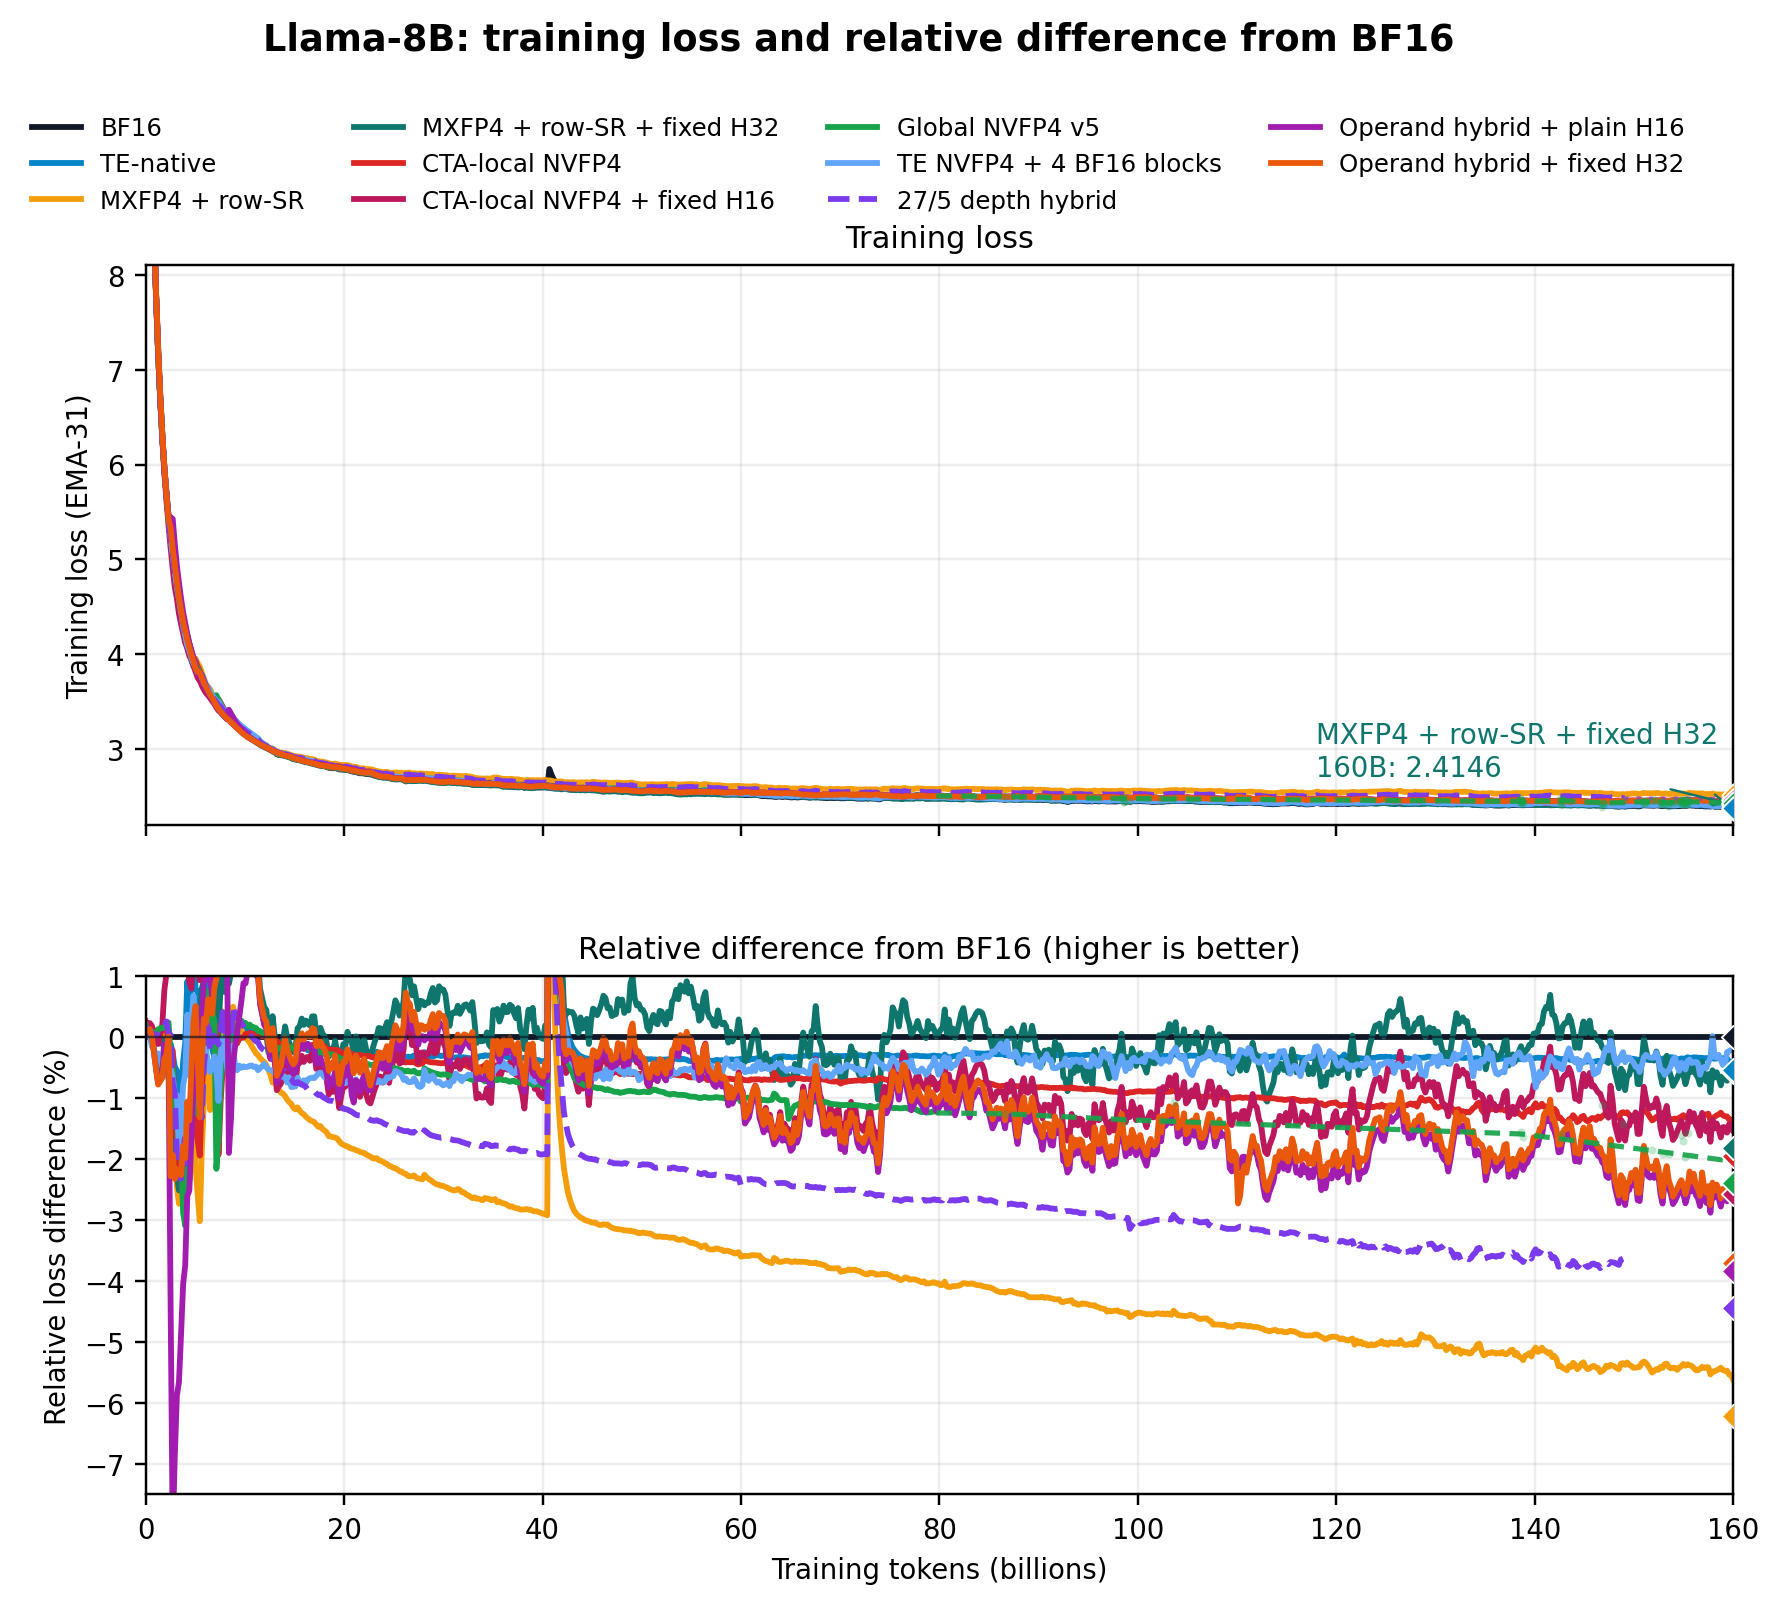
\includegraphics[width=0.98\textwidth]{figures/llama8b_160b_training_loss.png}
  \caption{Llama-8B training loss and relative difference from the BF16
  reference. Curves use EMA-31. Diamonds mark the final plotted endpoint.
  Sparse pure-v5 telemetry
  after step 19,000 is shown as exact anchors with a dashed robust locally
  weighted scatterplot smoothing (LOWESS) display fit. The fit is not used for
  endpoint values or comparisons. The dotted tail on the 27/5 depth hybrid
  marks a telemetry gap from its last continuous observations to the exact
  terminal point; it does not supply intermediate loss values.}
  \label{fig:llama8b-loss}
\end{figure}

Figure~\ref{fig:llama8b-loss-zoom} expands the final 40B-token window. It shows
the late loss separation at the same scale without extrapolating any route.

\begin{figure}[tbp]
  \centering
  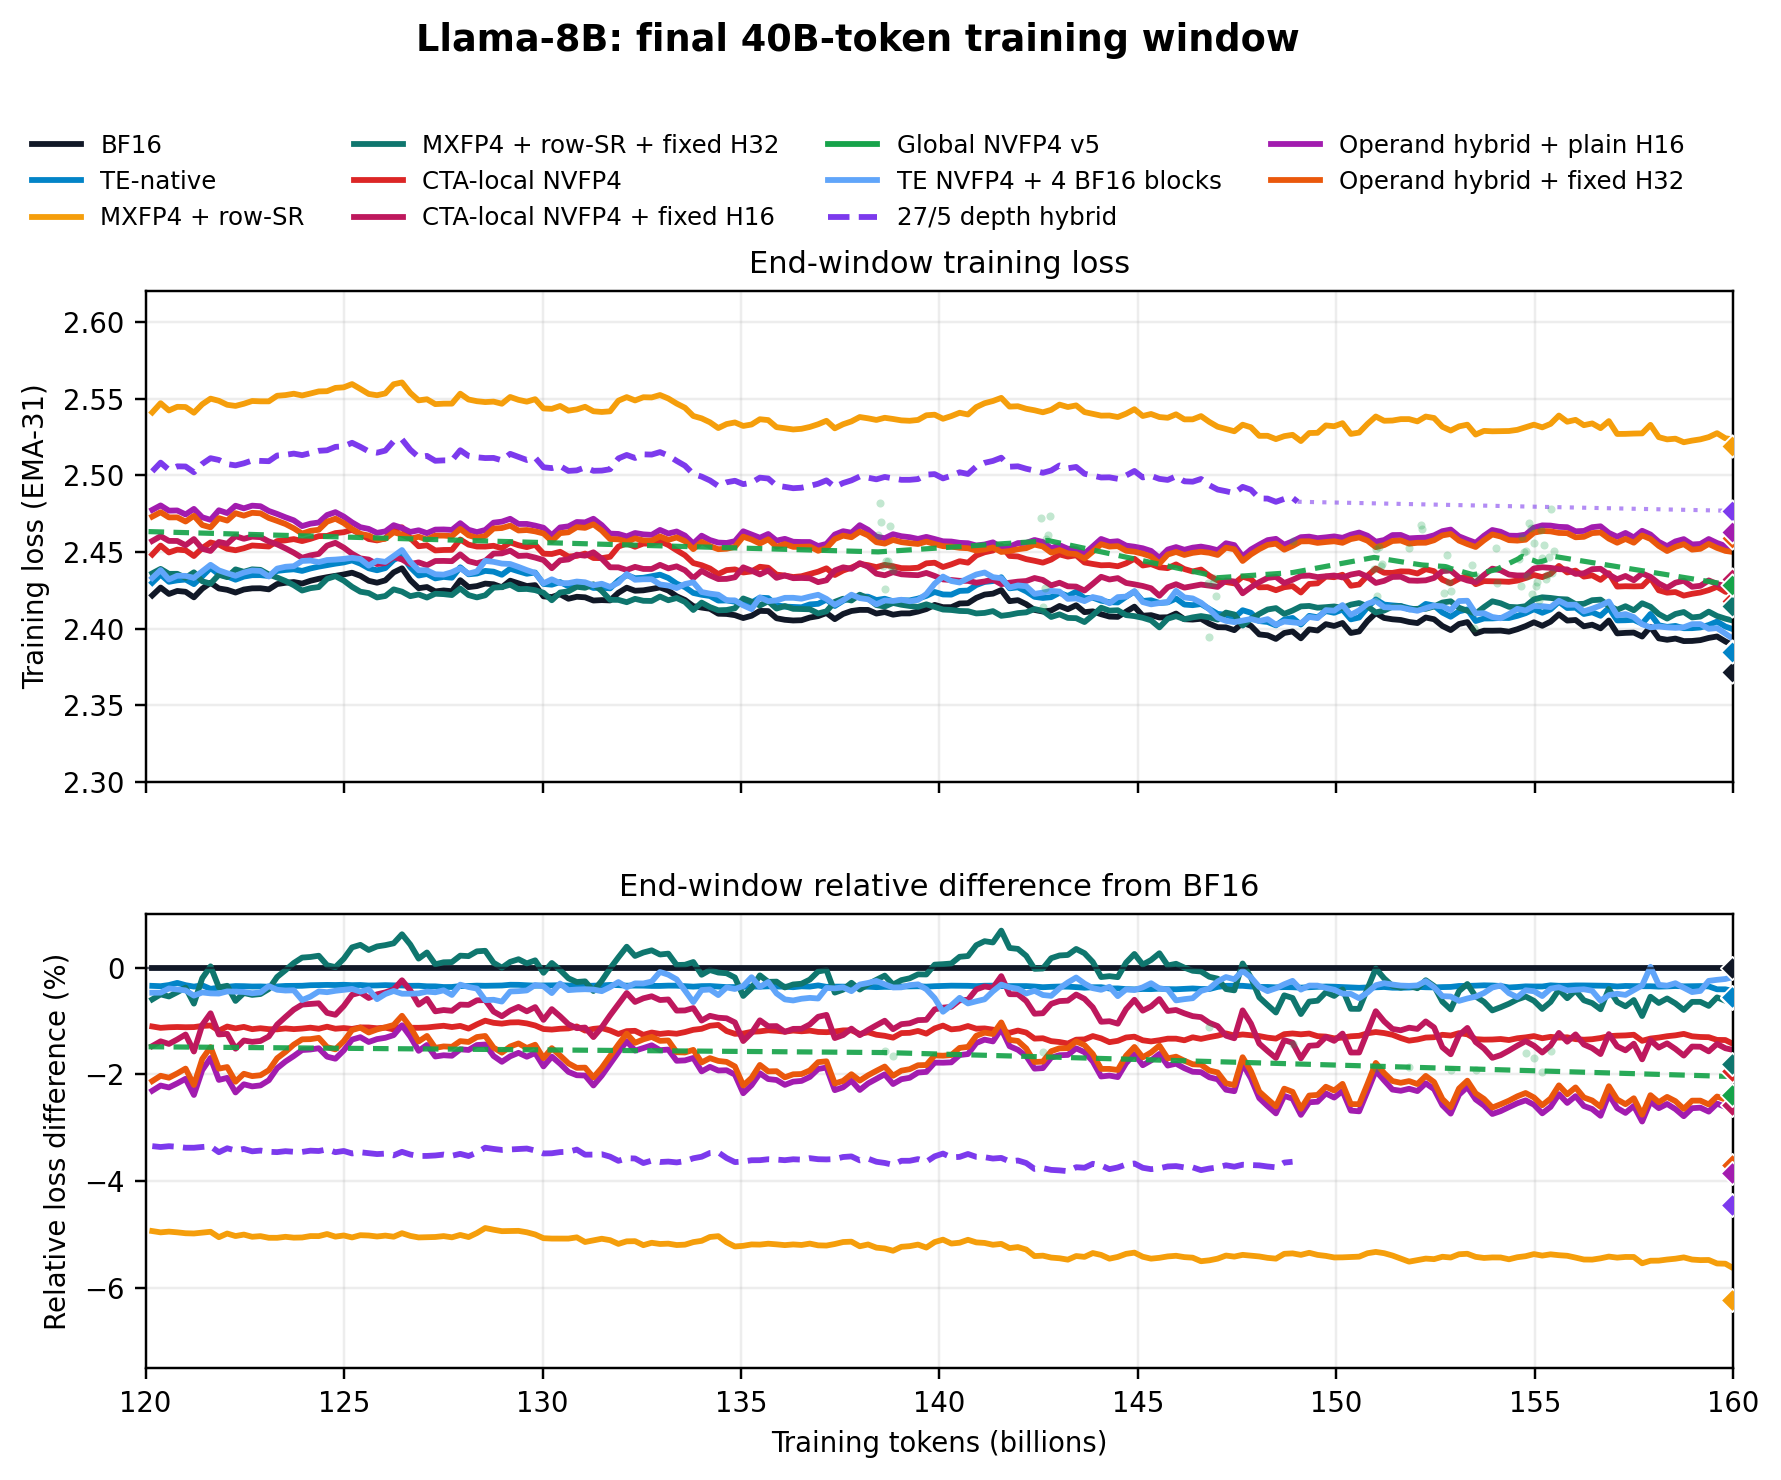
\includegraphics[width=0.98\textwidth]{figures/llama8b_160b_training_loss_zoom.png}
  \caption{Training loss from 120B to 160B tokens. Diamonds are exact logged
  endpoints. The dotted 27/5 tail marks an interval without intermediate
  telemetry and is not used in any comparison.}
  \label{fig:llama8b-loss-zoom}
\end{figure}

The TE route with four final BF16 blocks and the fixed-H32 operand hybrid each
contain 3,815 exact logged observations through step 38,140. Both trajectories
also have a sealed, resumable checkpoint at step 38,147.

\begin{table}[H]
  \centering
  \caption{Raw last logged minibatch loss at step 38,140 (159.97B tokens).
  ``Loss excess'' is relative to the unadjusted BF16 observation at that step.}
  \label{tab:training-endpoints}
  \begin{tabularx}{\textwidth}{Yrr}
    \toprule
    Route & Raw endpoint loss & Loss excess vs BF16 \\
    \midrule
    BF16 & 2.364637 & 0.00\% \\
    TE \nvfp{} + four final BF16 blocks & 2.385181 & 0.87\% \\
    TE-native \nvfp{} & 2.396353 & 1.34\% \\
    \mxfp{} + row-SR + fixed H32 & 2.414578 & 2.11\% \\
    \localcta{} & 2.417708 & 2.24\% \\
    Global \nvfp{} v5 & 2.428200 & 2.69\% \\
    \localcta{} + fixed H16 & 2.432642 & 2.88\% \\
    Operand hybrid + fixed H32 & 2.459305 & 4.00\% \\
    Operand hybrid + plain H16 & 2.462673 & 4.15\% \\
    27/5 depth hybrid & 2.476800 & 4.74\% \\
    \mxfp{} + row-SR & 2.519150 & 6.53\% \\
    \bottomrule
  \end{tabularx}
\end{table}

At step 38,140, the TE route with four final BF16 blocks is the closest
quantized trajectory to the raw BF16 observation, with 0.87\% excess, followed
by TE-native at 1.34\%. \mxfp{} with row-SR and fixed H32 is the closest custom
route at 2.11\%; it is 0.76\% above TE-native. The fixed-H32 operand hybrid
ends 1.85\% above the pure \mxfp{}-H32 route and 4.00\% above BF16.

Using tensors from the step-28,000 \mxfp{}+row-SR+fixed-H32 checkpoint, we replayed
Dgrad with \localcta{} and \mxfp{}. The surrounding replay configuration used
plain-H16 preconditioning only for Wgrad, which does not enter the scored
contraction. Against a BF16 replay, \localcta{} had lower Dgrad error energy
in all 288 layer--component comparisons; the geometric-mean
$E_{\mathrm{MX}}/E_{\mathrm{localCTA}}$ ratio was 1.292. The completed
plain-H16 operand hybrid nevertheless ends 1.99\% above \mxfp{}+row-SR+fixed H32 in
training loss. Appendix~\ref{app:dgrad-diagnostic} gives the capture and
aggregation contract.

\subsection{Validation loss}

Validation uses one fixed external stream with a complete document-and-token
provenance record. The converted and native evaluators agree exactly at the
full 8,192-token context. As a temporal control, BF16 validation NLL falls from
3.28327 at step 2,000 to 2.46052 at step 29,000. The paired difference is
$-0.82275$ NLL with a sequence-level standard error of 0.00371, placing the
comparison beyond the predeclared five-standard-error temporal gate. This
control establishes that the stream and evaluator recover the expected
learning order before comparing low-precision routes. Training loss is not
used as a substitute for validation loss.

Figure~\ref{fig:llama8b-validation} evaluates every available exact checkpoint
on that same stream. At the common step-38,000 cut, \mxfp{} with fixed H32 has
the lowest observed validation NLL, 2.422804. BF16 records 2.430206, the TE
route with four final BF16 blocks 2.437475, and TE-native 2.440488. The
fixed-H32 operand hybrid records 2.463842, compared with 2.460331 for
\localcta{} and 2.462074 for global \nvfp{} v5. Relative to BF16, the
\mxfp{}-H32, four-final-BF16-block, and operand-H32 differences are
$-0.305\%$, $+0.299\%$, and $+1.384\%$, respectively. These are observed
single-trajectory comparisons, not a one-factor isolation of H32 or
repeated-seed estimates.

\begin{figure}[tbp]
  \centering
  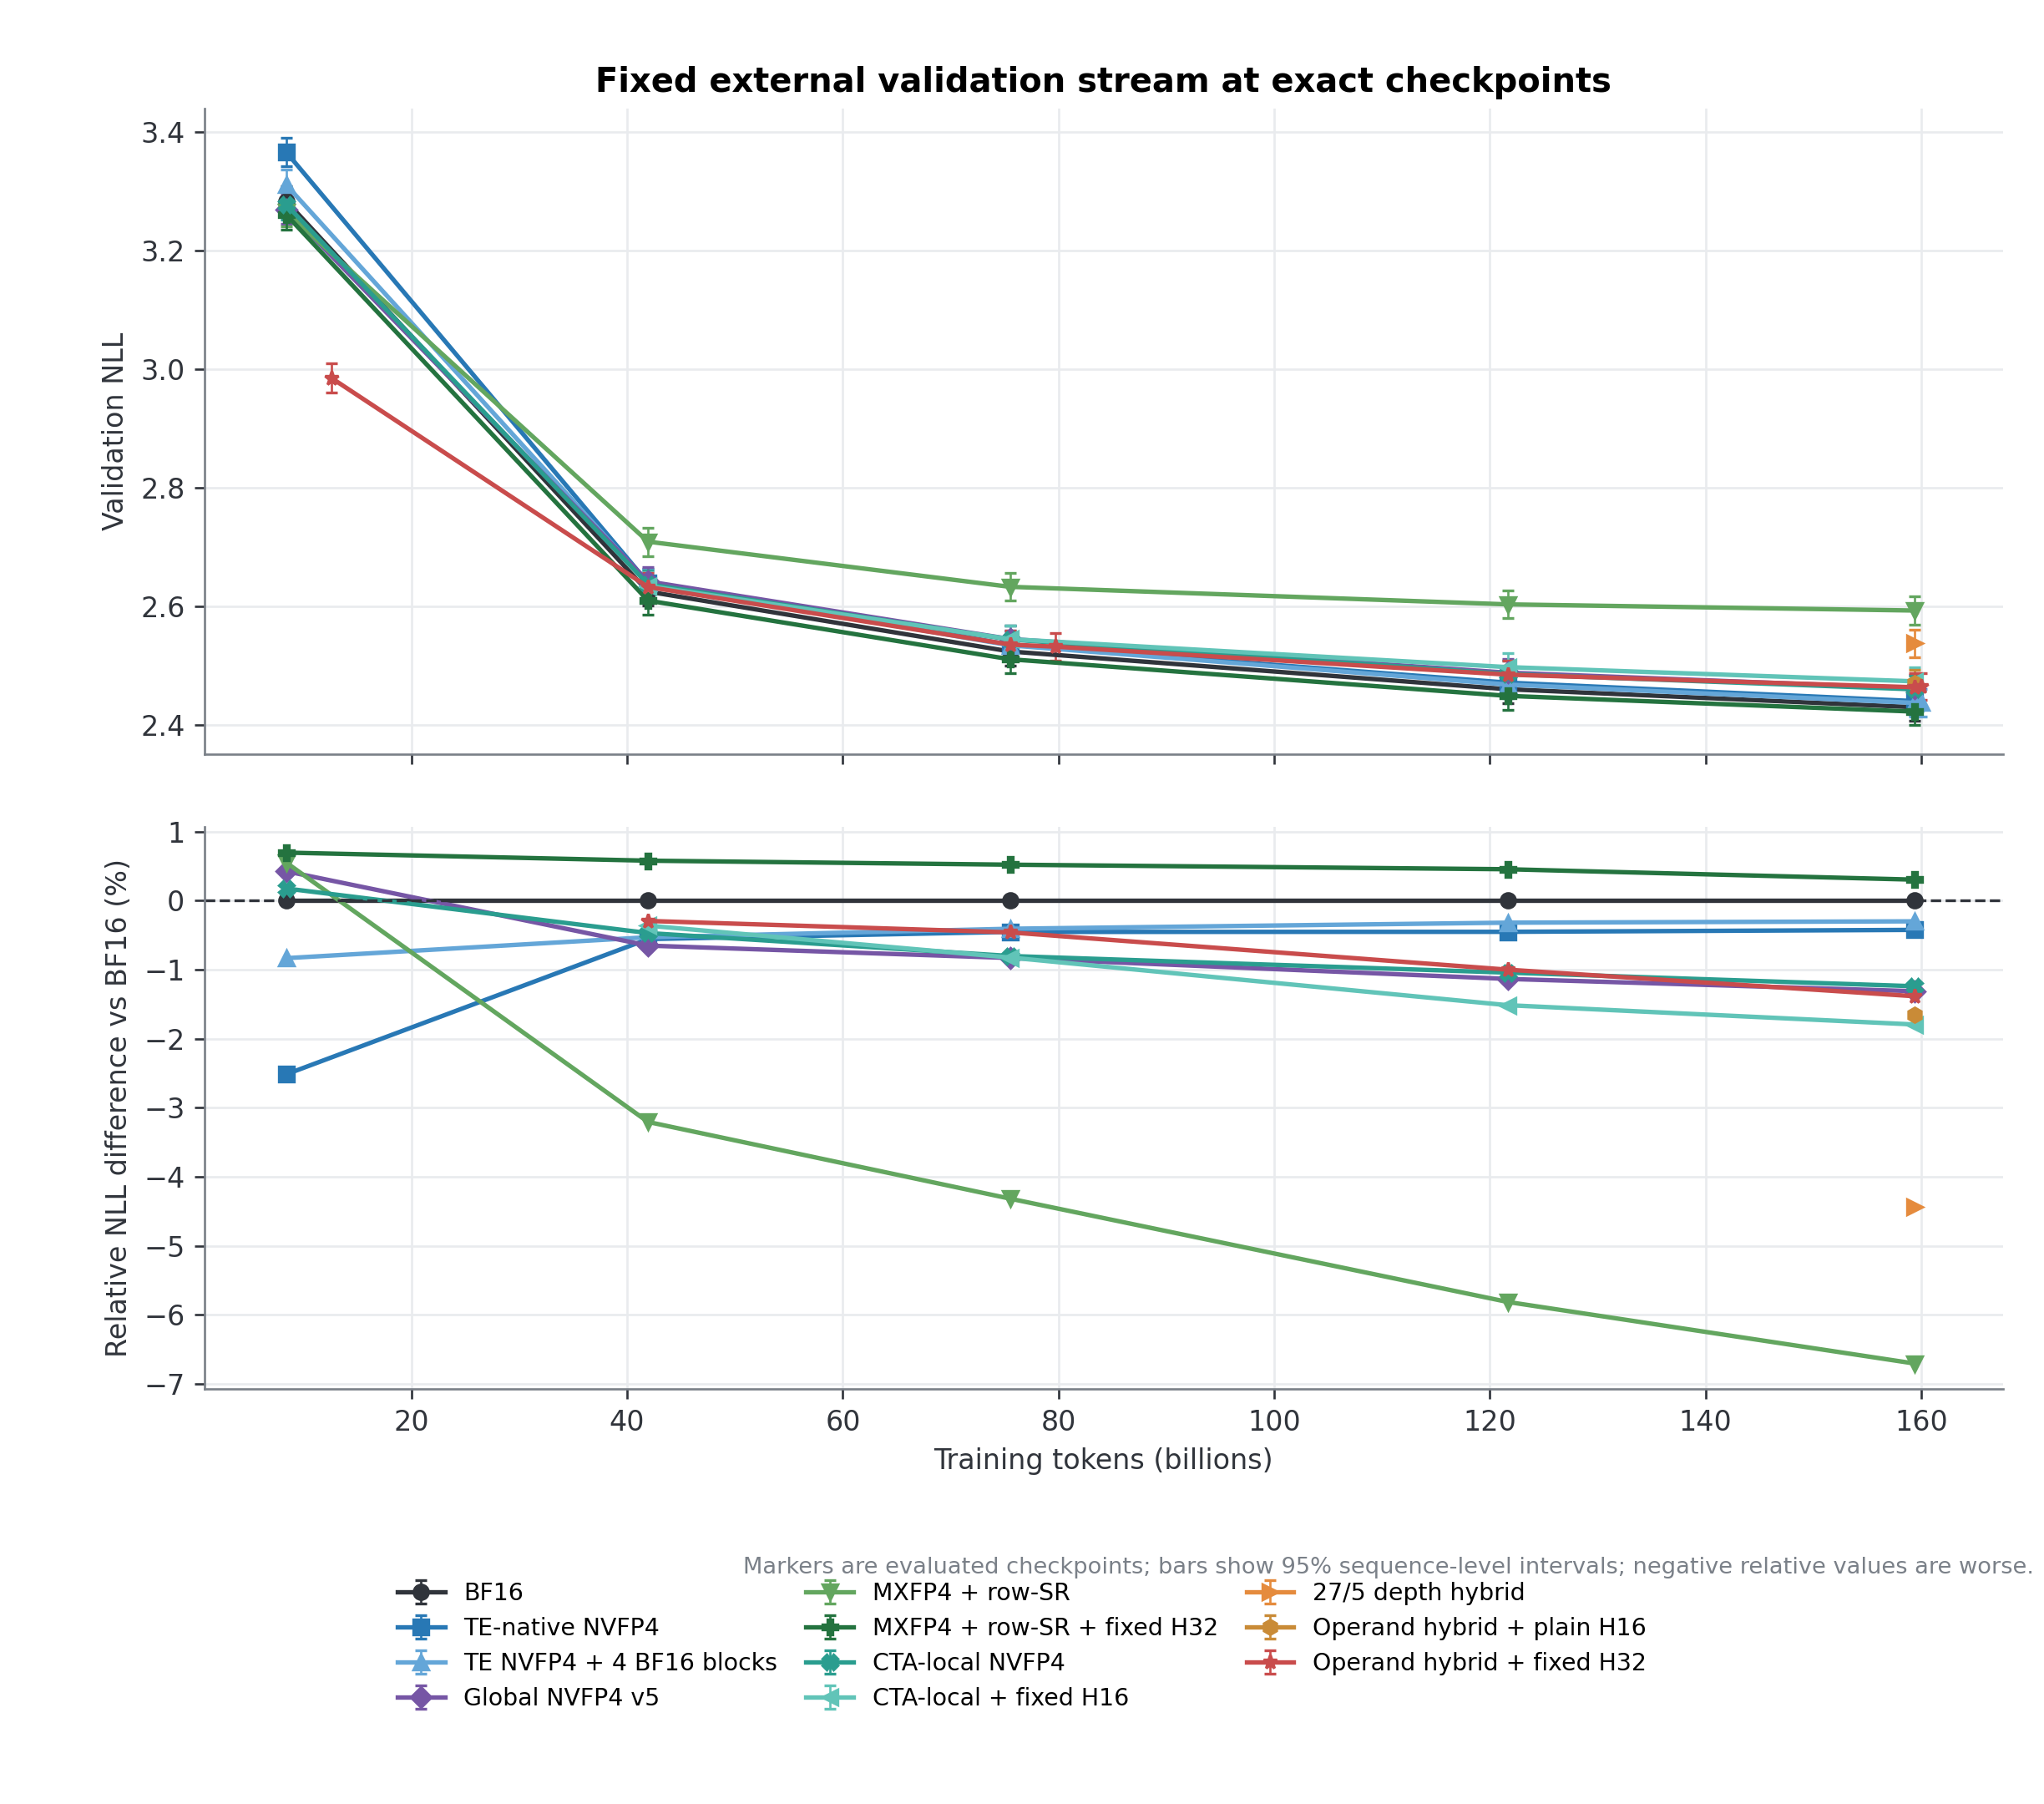
\includegraphics[width=0.98\textwidth]{figures/llama8b_validation_nll.png}
  \caption{Validation NLL on the fixed external stream at every available exact
  checkpoint. Error bars are 95\% sequence-level intervals. The lower panel
  reports $100(L_{\mathrm{BF16}}-L_{\mathrm{route}})/L_{\mathrm{BF16}}$ at
  exact shared steps, so negative values are worse than BF16. Lines connect
  measured checkpoints only; missing checkpoints are neither interpolated nor
  extrapolated.}
  \label{fig:llama8b-validation}
\end{figure}

\FloatBarrier

\subsection{How do the routes compare on downstream tasks?}

Each route is evaluated from its complete step-38,000 checkpoint using BF16
inference after verifying agreement with the training RoPE and RMSNorm
definitions. Eleven routes meet these criteria; routes without a complete
step-38,000 checkpoint are omitted. Every route uses the same MMLU,
HellaSwag, WinoGrande, and ARC-Challenge protocol.

\begin{table}[htbp]
  \centering
  \footnotesize
  \caption{Exact step-38,000 downstream scores (\%). MMLU and WinoGrande
  report accuracy; HellaSwag and ARC-Challenge report normalized accuracy.
  Shot counts are 5, 10, 5, and 25, respectively. Every route uses BF16
  inference after exact converted/native parity.}
  \label{tab:downstream-step38}
  \begin{adjustbox}{max width=\textwidth}
  \begin{tabular}{lrrrr}
    \toprule
    Route & MMLU & HellaSwag & WinoGrande & ARC-Challenge \\
    \midrule
    \input{data/llama8b_scaledrope_downstream_table_rows_20260903.tex}
  \end{tabular}
  \end{adjustbox}
\end{table}

The task ordering is not uniform. BF16 has the highest MMLU score, the
fixed-H32 operand hybrid has the highest WinoGrande score, and
\mxfp{}+row-SR+fixed H32 has the highest HellaSwag and ARC-Challenge scores.
Relative to that pure \mxfp{}-H32 route, the fixed-H32 operand hybrid differs
by $-1.66$, $-2.02$, $+0.79$, and $-2.39$ points on MMLU, HellaSwag,
WinoGrande, and ARC-Challenge, respectively. The four-final-BF16-block TE
route differs from BF16 by $-2.19$, $-0.53$, $-1.10$, and $+1.19$ points.
These are observations from one checkpoint per trajectory, not repeated-seed
estimates.

\begin{figure}[htbp]
  \centering
  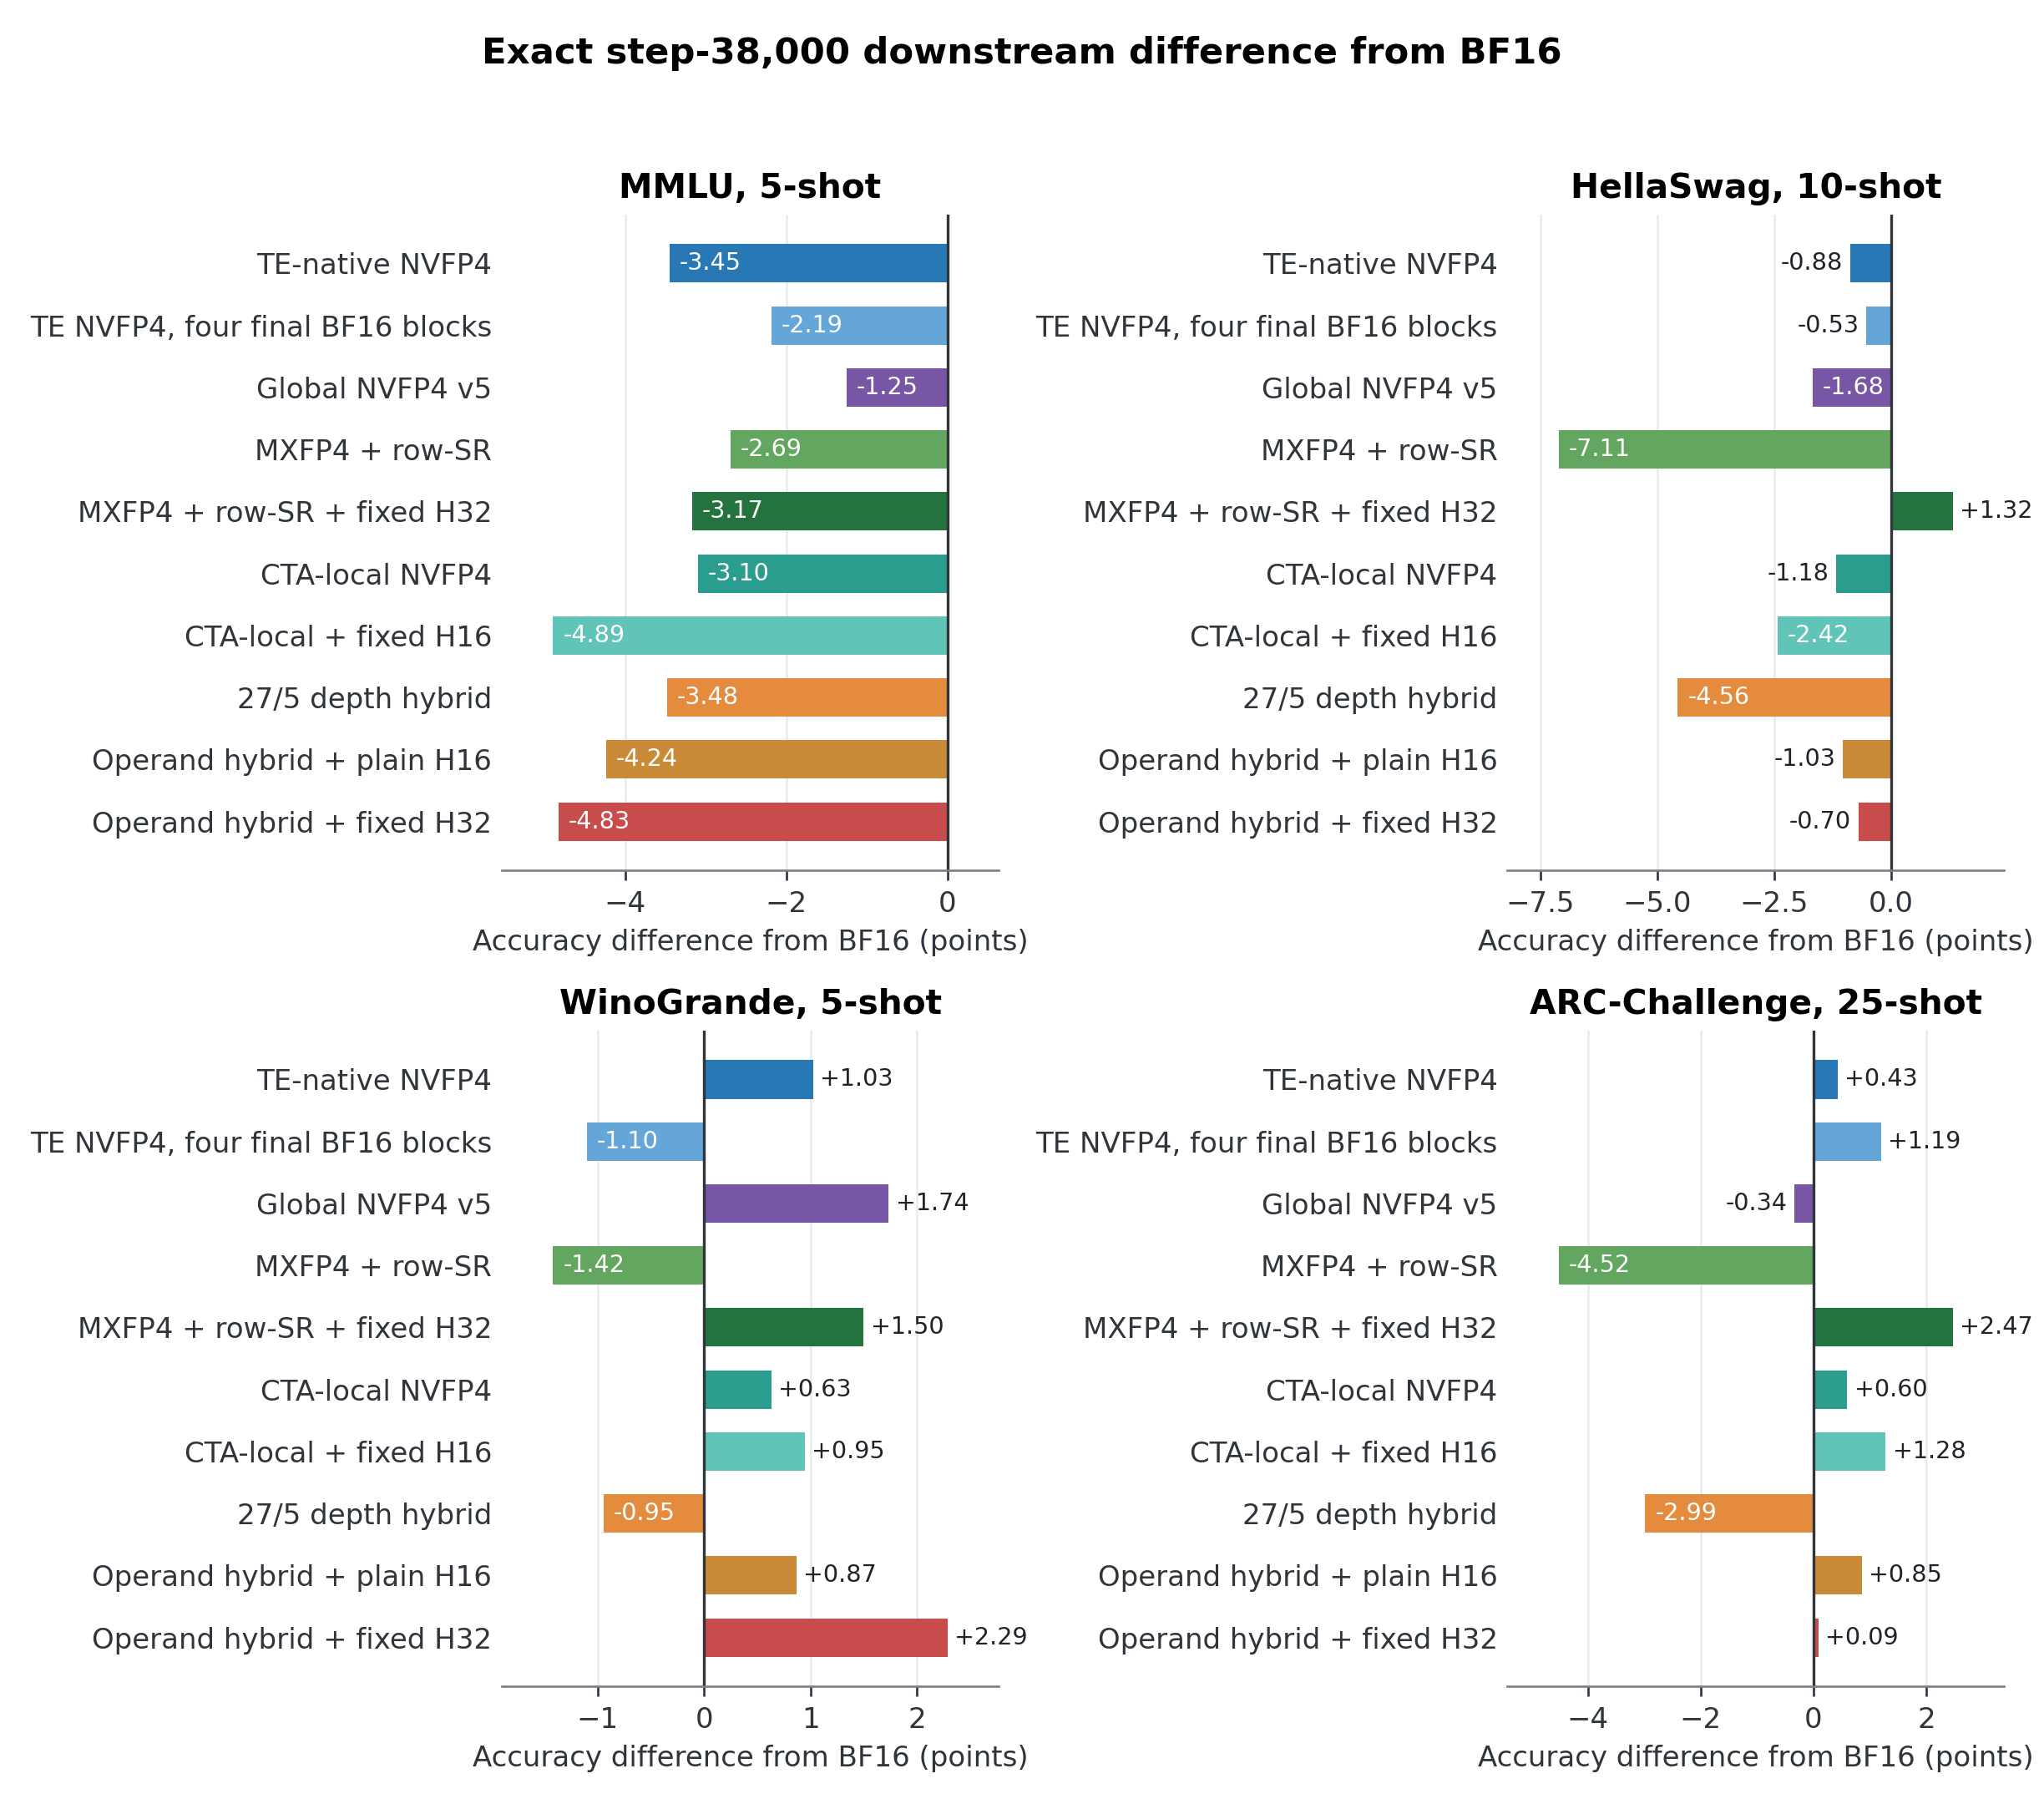
\includegraphics[width=0.98\textwidth]{figures/fp4_downstream_delta_bf16.png}
  \caption{Downstream reported-score difference from BF16 at exact step 38,000.
  Positive values exceed the BF16 score on that task. The absolute scores are
  reported in Table~\ref{tab:downstream-step38}.}
  \label{fig:downstream-delta}
\end{figure}
\FloatBarrier
